\documentclass[krantz2]{krantz}%,ChapterTOCs

%\usepackage[utf8]{inputenc}
\usepackage{color}

\usepackage{polyglossia}
\setdefaultlanguage[variant = british, ordinalmonthday = false]{english}

%\usepackage{gitinfo2} % remember to setup Git hooks

\usepackage{hologo}

\usepackage{csquotes}

\usepackage{graphicx}
\DeclareGraphicsExtensions{.jpg,.pdf,.png}

\usepackage{animate}

%\usepackage{microtype}
\usepackage[style=authoryear-comp,giveninits,sortcites,maxcitenames=2,%
    mincitenames=1,maxbibnames=10,minbibnames=10,backref,uniquename=mininit,%
    uniquelist=minyear,sortgiveninits=true,backend=biber]{biblatex}%,refsection=chapter

\newcommand{\href}[2]{\emph{#2} (\url{#1})}

%\usepackage[unicode,hyperindex,bookmarks,pdfview=FitB,%backref,
%            pdftitle={Learn R ...as you learnt your mother tongue},%
%            pdfkeywords={R, statistics, data analysis, plotting},%
%            pdfsubject={R},%
%            pdfauthor={Pedro J. Aphalo}%
%            ]{hyperref}

%\hypersetup{colorlinks,breaklinks,
%             urlcolor=blue,
%             linkcolor=blue,
%             citecolor=blue,
%             filecolor=blue,
%             menucolor=blue}

\usepackage{framed}

\usepackage{abbrev}
\usepackage{usingr}

\usepackage{imakeidx}

% this is to reduce spacing above and below verbatim, which is used by knitr
% to show returned values
\usepackage{etoolbox}
\makeatletter
\preto{\@verbatim}{\topsep=-5pt \partopsep=-4pt \itemsep=-2pt}
\makeatother

%%% Adjust graphic design

% New float "example" and corresponding "list of examples"
%\DeclareNewTOC[type=example,types=examples,float,counterwithin=chapter]{loe}
%\DeclareNewTOC[name=Box,listname=List of Text Boxes, type=example,types=examples,float,counterwithin=chapter,%
%]{lotxb}

% changing the style of float captions
%\addtokomafont{caption}{\sffamily\small}
%\setkomafont{captionlabel}{\sffamily\bfseries}
%\setcapindent{0em}

% finetuning tocs
%\makeatletter
%\renewcommand*\l@figure{\@dottedtocline{1}{0em}{2.6em}}
%\renewcommand*\l@table{\@dottedtocline{1}{0em}{2.6em}}
%\renewcommand*\l@example{\@dottedtocline{1}{0em}{2.3em}}
%\renewcommand{\@pnumwidth}{2.66em}
%\makeatother
%
%% add pdf bookmarks to tocs
%\makeatletter
%\BeforeTOCHead{%
%  \cleardoublepage
%    \edef\@tempa{%
%      \noexpand\pdfbookmark[0]{\list@fname}{\@currext}%
%    }\@tempa
%}

\setcounter{topnumber}{3}
\setcounter{bottomnumber}{3}
\setcounter{totalnumber}{4}
\renewcommand{\topfraction}{0.90}
\renewcommand{\bottomfraction}{0.90}
\renewcommand{\textfraction}{0.10}
\renewcommand{\floatpagefraction}{0.70}
\renewcommand{\dbltopfraction}{0.90}
\renewcommand{\dblfloatpagefraction}{0.70}

\addbibresource{rbooks.bib}
\addbibresource{references.bib}

\makeindex

\begin{document}

% customize chapter format:
%\KOMAoption{headings}{twolinechapter}
%\renewcommand*\chapterformat{\thechapter\autodot\hspace{1em}}

% customize dictum format:
%\setkomafont{dictumtext}{\itshape\small}
%\setkomafont{dictumauthor}{\normalfont}
%\renewcommand*\dictumwidth{0.7\linewidth}
%\renewcommand*\dictumauthorformat[1]{--- #1}
%\renewcommand*\dictumrule{}

%\extratitle{\vspace*{2\baselineskip}%
%             {\Huge\textsf{\textbf{Learn R}\\ \textsl{\huge\ldots as you learnt your mother tongue}}}}

\title{\Huge{\fontseries{ub}\sffamily Learn R\\{\Large\ldots as you learnt your mother tongue}}}

%\subtitle{Git hash: \gitAbbrevHash; Git date: \gitAuthorIsoDate}

\author{Pedro J. Aphalo}

\date{Helsinki, \today}

%\publishers{Draft, 95\% done\\Available through \href{https://leanpub.com/learnr}{Leanpub}}

%\uppertitleback{\copyright\ 2001--2017 by Pedro J. Aphalo\\
%Licensed under one of the \href{http://creativecommons.org/licenses/}{Creative Commons licenses} as indicated, or when not explicitly indicated, under the \href{http://creativecommons.org/licenses/by-sa/4.0/}{CC BY-SA 4.0 license}.}
%
%\lowertitleback{Typeset with \href{http://www.latex-project.org/}{\hologo{XeLaTeX}}\ in Lucida Bright and \textsf{Lucida Sans} using the KOMA-Script book class.\\
%The manuscript was written using \href{http://www.r-project.org/}{R} with package knitr. The manuscript was edited in \href{http://www.winedt.com/}{WinEdt} and \href{http://www.rstudio.com/}{RStudio}.
%The source files for the whole book are available at \url{https://bitbucket.org/aphalo/using-r}.}

%\frontmatter

% knitr setup















% \thispagestyle{empty}
% \titleLL
% \clearpage

\frontmatter

\maketitle

%\begin{titlingpage}
%  \maketitle
%\titleLL
%\end{titlingpage}

\setcounter{page}{7} %previous pages will be reserved for frontmatter to be added in later.
\tableofcontents
%\chapter*{Foreword}
I am delighted to introduce the first book on Multimedia Data Mining.  When I came to know about this book project undertaken by two of the most active young researchers in the field, I was pleased that this book is coming in early stage of a field that will need it more than most fields do.  In most emerging research fields, a book can play a significant role in bringing some maturity to the field.  Research fields advance through research papers.  In research papers, however, only a limited perspective could be provided about the field, its application potential, and the techniques required and already developed in the field.  A book gives such a chance.  I liked the idea that there will be a book that will try to unify the field by bringing in disparate topics already available in several papers that are not easy to find and understand.  I was supportive of this book project even before I had seen any material on it.  The project was a brilliant and a bold idea by two active researchers.  Now that I have it on my screen, it appears to be even a better idea.  

Multimedia started gaining recognition in 1990s as a field.  Processing, storage, communication, and capture and display technologies had advanced enough that researchers and technologists started building approaches to combine information in multiple types of signals such as audio, images, video, and  text.  Multimedia computing and communication techniques recognize correlated information in multiple sources as well as insufficiency of information in any individual source.    By properly selecting sources to provide complementary information, such systems aspire, much like human perception system, to create a holistic picture of a situation using only partial information from separate sources.

Data mining is a direct outgrowth of progress in data storage and processing speeds.  When it became possible to store large volume of data and run different statistical computations to explore all possible and even unlikely correlations among data, the field of data mining was born.  Data mining allowed people to hypothesize relationships among data entities and explore support for those.  This field has been put to applications in many diverse domains and keeps getting more applications.  In fact many new fields are direct outgrowth of data mining and it is likely to become a powerful computational tool.\vadjust{\vfill\pagebreak}



\chapter*{Preface}

\begin{VF}
``Suppose that you want to teach the `cat' concept to a very young child. Do you explain that a cat is a relatively small, primarily carnivorous mammal with retractible claws, a distinctive sonic output, etc.? I'll bet not. You probably show the kid a lot of different cats, saying `kitty' each time, until it gets the idea. To put it more generally, generalizations are best made by abstraction from experience.''

\VA{R. P. Boas}{Can we make mathematics intelligible?}
\end{VF}

%\dictum[R. P. Boas (1981) Can we make mathematics intelligible?, \emph{American Mathematical Monthly} \textbf{88:} 727-731.]{"Suppose that you want to teach the `cat' concept to a very young child. Do you explain that a cat is a relatively small, primarily carnivorous mammal with retractible claws, a distinctive sonic output, etc.? I'll bet not. You probably show the kid a lot of different cats, saying `kitty' each time, until it gets the idea. To put it more generally, generalizations are best made by abstraction from experience."}


% Such pauses are not a miss use of our time. To learn a natural language we need to interact with other speakers, we need feedback. In the case of R, we can get feedback both from the outcomes from our utterances to the computer, and from other \Rlang users.}
\noindent
This book covers different aspects of the use of the \Rlang language. Chapters \ref{chap:R:introduction} to \ref{chap:R:functions} describe the \Rlang language itself. Later chapters describe extensions to the \Rlang language available through contributed \emph{packages}, the \emph{grammar of data} and the \emph{grammar of graphics}. In this book, explanations are concise but contain pointers to additional sources of information, so as to encourage the development of a routine of independent exploration. This is not an arbitrary decision, this is the normal \emph{modus operandi} of most of us who use \Rlang regularly for a variety of different problems. Some have called approaches like the one used here, ``learning the hard way'', but I would call it ``learning to be independent''.

I do not discuss in this book statistics or data analysis methods, I describe \Rlang as a language for data manipulation and display. The idea is for you to learn the \Rlang language in a way comparable to how children learn a language: they work-out what the rules are, simply by listening to people speak and trying to utter what they want to tell their parents. Of course, small children receive some guidance, but are not taught a prescriptive set of rules like when learning a second language at school. Instead of listening, you will read code and instead of speaking you will try to execute \Rlang  code statements on a computer---i.e. you will try your hand at using \Rlang to tell a computer what you want it to compute. I do provide explanations and guidance, but the idea of this book is for you to use the numerous examples to find-out by yourself the overall patterns and coding philosophy behind the \Rlang language. Instead of parents being the sound board for your first utterances in \Rlang, the computer will play this role. You will \emph{play} by modifying the examples, see how the computer responds, does \Rlang understand you or not? Using actively a language is the most efficient way of learning it. By using it, I mean actually reading, writing and running scripts or programs (copying and pasting, or typing ready-made examples from books or the internet does not qualify as using a language).

What is a language? A language is a system of communication. \Rlang as a language allows us to communicate with other members of the \Rlang community, and with computers. As most languages in active use, \Rlang evolves. New ``words'' and new ``constructs'' are incorporated into the language, and some earlier frequently used ones are relegated to the fringes of the corpus. I describe current usage and ``modisms'' of the \Rlang language in a way accessible to a readership unfamiliar with computer science but with some background in data analysis as used in Biology, Engineering, or Humanities.

When teaching I tend to lean towards challenging students rather than telling an over-simplified story. There are two reasons for this. First, I prefer as a student, and I learn best myself if the going is not too easy. Second, if I would hide the tricky bits of the \Rlang language, it would make readers' life much more difficult later on. You, will not remember all the details, nobody could. However, you most likely will remember in which situations you need to be careful or should check the details. So, I will expose you not only the usual cases, but also to several exceptions and counterintuitive features of the language. Reading this book will be about exploring a new world, this book aims to be a travel guide, but neither a traveler's account, nor a cookbook of \Rlang recipes.

Keep in mind that it is impossible to remember everything about \Rlang! The \Rlang language in a broad sense is vast because its capabilities can be expanded with independently developed packages. Learning to use \Rlang consists in learning the basics plus developing the skill of finding your way in \Rlang and its documentation.  In 2017 the number packages available in the Comprehensive \Rlang Archive Network (CRAN) broke the 10\,000 barrier. CRAN is the most important, but not only, public repository for \Rlang packages. How good a command of the \Rlang language and packages a user needs depends on the type activities to be carried out. This book attempts to train you in the use of the \Rlang language itself and of popular \Rlang language extensions for data manipulation and graphical display. Given the availability of numerous books on statistical analysis with \Rlang, in the present book I will cover only the bare minimum of this subject. The same is true for package development in \Rlang. This book seats in-between, aiming at teaching programming in-the-small: the use of \Rlang to automate the drudgery of data manipulation from raw data, through data exploration to the production of publication quality illustrations.

As with all ``rich'' languages there are many different ways of doing things in \Rlang, and there is in almost all cases no one-size-fits-all solution to a problem. There is always a compromise involved, usually between time spent by the user and processing time required in the computer. Many of the packages that are most popular nowadays did not exist when I started using \Rlang, and many of these packages make new approaches available. One could write many different \Rlang books with a given aim using substantially different ways of achieving the same results. In this book, I limit myself to packages that are currently popular and/or that I consider elegantly designed. I have in particular tried to limit myself to packages with similar design philosophies, especially in relation to their interfaces. What is elegant design, and in particular what is a friendly user interface depends strongly on each user's preferences and previous experience. Consequently, the contents of the book are strongly biased by my own preferences. I have tried to write examples in ways that execute fast without compromising readability. I encourage readers to take this book as a starting point for exploring the very many packages, styles and approaches which I have not described.

I will appreciate suggestions for further examples, notification of errors and unclear sections. Many of the examples here have been collected from diverse sources over many years and because of this not all sources are acknowledged. If you recognize any example as yours or someone else's please let me know so that I can add a proper acknowledgement. I warmly thank the students that over the years have asked the questions and posed the problems that have helped me write this text and correct the mistakes and voids of previous versions. I have also received help on on-line forums and in person from numerous people, learnt from archived e-mail list messages, blog posts, books, articles, tutorials, webinars, and by struggling to solve some new problems on my own. In many ways this text owes much more to people who are not authors than to myself. However, as I am the one who has written this version and decided what to include and exclude, as author, I take full responsibility for any errors and inaccuracies.

I have been using \Rlang since around 1998 or 1999, but I am still constantly learning new things about \Rlang itself and \Rlang packages. With time it has replaced in my work as a researcher and teacher several other pieces of software: \pgrmname{SPSS}, \pgrmname{Systat}, \pgrmname{Origin}, \pgrmname{Excel}, and it has become a central piece of the tool set I use for producing lecture slides, notes, books and even web pages. This is to say that it is the most useful piece of software and programming language I have ever learnt to use. Of course, in time it will be replaced by something better, but at the moment it is a key language to learn for anybody with a need to analyse and display data.

Why the title ``\emph{Learn R \ldots as you learnt your mother tongue}''? On one hand, because this book is based on exploration and practice. On the other hand, because you will be exposed to current usage and not spared the quirks of the language. When we use our mother tongue in everyday life we do not think about grammar rules or sentence structure, except for the trickier or unfamiliar situations. My aim is for this book to help you grow to use \Rlang in this same way.

\begin{framed}
\noindent\large%
\textbf{I encourage you to approach R, like a child approaches his or hers mother tongue when learning to speak:} Do not struggle, just play! If going gets difficult and frustrating, take a break! If you get a new insight, take a break to enjoy the victory!
\end{framed}

\newpage

\begin{framed}
\noindent
\textbf{Icons used to mark different content.} Throughout the book text boxes marked with icons present different types of information. First of all, we have \emph{playground} boxes indicated with \playicon\ which contain open-ended exercises---ideas and pieces of \Rlang code to play with at the \Rlang console. A few of these will require more time to grasp, and are indicated with \advplayicon. Boxes providing general information, usually not directly related to \Rlang as a language, are indicated with \infoicon. Some boxes highlighted with \ilAttention\ give important bits of information that must be remembered when using \Rlang---i.e.\ explain some unusual feature of the language. Finally, some boxes indicated by \ilAdvanced\ give in depth explanations, that may require you to spend time thinking, which en general can be skipped on first reading, but to which you should return at a later, and peaceful, time with a cup of coffee or tea.
\end{framed}
\newpage

%\newpage
%\begin{infobox}
%\noindent
%\textbf{Status as of 2016-11-23.} I have updated the manuscript to track package updates since the previous version uploaded six months ago, and added several examples of the new functionality added to packages \ggpmisc, \ggrepel, and \ggplot. I have written new sections on packages \viridis, \pkgname{gganimate}, \pkgname{ggstance}, \pkgname{ggbiplot}, \pkgname{ggforce}, \pkgname{ggtern} and \pkgname{ggalt}. Some of these sections are to be expanded, and additional sections are planned for other recently released packages.
%
%With respect to the chapter \textit{Storing and manipulating data with R} I have put it on hold, except for the introduction, until I can see a soon to be published book covering the same subject. Hadley Wickham has named the set of tools developed by him and his collaborators as \textit{tidyverse} to be described in the book titled \textit{R for Data Science} by Grolemund and Wickham (O'Reilly).
%
%An important update to \ggplot was released last week, and it includes changes to the behavior of some existing functions, specially faceting has become extensible through other packages. Several of the new facilities are described in the updated text and code included in this book and this pdf has been generated with up-to-date version of \ggplot and packages as available today from CRAN, except for \pkgname{ggtern} which was downloaded from Bitbucket minutes ago.
%
%The present update adds about 100 pages to the previous versions. I expect to upload a new update to this manuscript in one or two months time.
%
%\textbf{Status as of 2017-01-17.} Added ``playground'' exercises to the chapter describing \ggplot, and converted some of the examples earlier part of the main text into these playground items. Added icons to help readers quickly distinguish playground sections (\textcolor{blue}{\noticestd{"0055}}), information sections (\textcolor{blue}{\modpicts{"003D}}), warnings about things one needs to be specially aware of (\colorbox{yellow}{\typicons{"E136}}) and boxes with more advanced content that may require longer time/more effort to grasp (\typicons{"E04E}). Added to the sections \code{scales} and examples in the \ggplot chapter details about the use of colors in \Rlang and \ggplot2. Removed some redundant examples, and updated the section on \code{plotmath}. Added terms to the alphabetical index. Increased line-spacing to avoid uneven spacing with inline code bits.
%
%\textbf{Status as of 2017-02-09.} Wrote section on ggplot2 themes, and on using system- and Google fonts in ggpplots with the help of package \pkgname{showtext}. Expanded section on \ggplot's \code{annotation}, and revised some sections in the ``R scripts and Programming'' chapter. Started writing the data chapter. Wrote draft on writing and reading text files. Several other smaller edits to text and a few new examples.
%
%\textbf{Status as of 2017-02-14.} Wrote sections on reading and writing MS-Excel files, files from statistical programs such as SPSS, SyStat, etc., and NetCDF files. Also wrote sections on using URLs to directly read data, and on reading HTML and XML files directly, as well on using JSON to retrieve measured/logged data from IoT (internet of things) and similar intelligent physical sensors, micro-controller boards and sensor hubs with network access.
%
%\textbf{Status as of 2017-03-25.} Revised and expanded the chapter on plotting maps, adding a section on the manipulation and plotting of image data. Revised and expanded the chapter on extensions to \pkgname{ggplot2}, so that there are no longer empty sections. Wrote short chapter ``If and when \Rlang needs help''. Revised and expanded the ``Introduction'' chapter. Added index entries, and additional citations to literature.
%
%\textbf{Status as of 2017-04-04.} Revised and expanded the chapter on using \Rpgrm as a calculator. Revised and expanded the ``Scripts'' chapter. Minor edits to ``Functions'' chapter. Continued writing chapter on data, writing a section on \Rlang native apply functions and added preliminary text for a pipes and tees section. Write intro to `tidyverse' and grammar of data manipulation. Added index entries, and a few additional citations to the literature. Spell checking.
%
%\textbf{Status as of 2017-04-08.} Completed writing first draft of chapter on data, writing all the previously missing sections on the ``grammar of data manipulation''. Wrote two extended examples in the same chapter. Add table listing several extensions to \pkgname{ggplot2} not described in the book.
%
%\textbf{Status as of 2017-04-13.} Revised all chapters correcting some spelling mistakes, adding some explanatory text and indexing all functions and operators used. Thoroughly revised the Introduction chapter and the Preface. Expanded section on bar plots (now bar and column plots). Revised section on tile plots. Expanded section on factors in chapter 2, adding examples of reordering of factor labels, and making clearer the difference between the labels of the levels and the levels themselves.
%
%\textbf{Status as of 2017-04-29.} Tested with R 3.4.0. Package \pkgname{gganimate} needs to be installed from Github as the updated version is not yet in CRAN. Function \code{gg\_animate()} has been renamed \code{gganimate().}
%
%\textbf{Status as of 2017-05-14.} Submitted package \pkgname{learnrbook} to CRAN. Revised code in the book
%to use this new package. Small fixes after more testing. Added examples of plotting and labeling based on fits with \code{method = "nls"}, including use of the new \code{ggpmisc::stat\_fit\_tidy()}.
%
%\textbf{Status as of 2017-06-11.} Added sections on R-code bench marking and profiling for performance optimization. Added also an example of explicit compilation of a function defined in the R language. Added section on functions \code{assign()}, \code{get()} and \code{mget()}.
%
%\textbf{Status as of 2017-08-12.} Various edits to all chapters. Expanded section on \pkgname{ggpmisc} to include the new functionality added in version 0.2.15.9002: \code{geom\_table} and \code{stat\_fit\_tb}. Added section on package \pkgname{ggbeeswarm}. Added sections on packages \pkgname{magick} and on using \pgrmname{ImageJ} from \Rpgrm. Improved indexing and cross references.
%
%\textbf{Status as of 2017-10-25.} Edited the chapter on using R as a calculator, adding examples on insertion and deletion of members of lists and vectors, and also of use of \code{gl()} and \code{reorder()}. Edited sections on scale limits and added new section on coordinate limits to explain more thoroughly their differences and uses in chapter on plotting with \pkgname{ggplot2}. Added a section on package \pkgname{ggsignif} to the chapter on extensions to \pkgname{ggplot2}. Expanded section on \pkgname{ggpmisc} in the same chapter describing new functionality added in version 0.2.16.
%\pkgname{ggplo2} $>=$ 2.2.1.9000 is required by the current development version of \pkgname{ggpmisc}.
%
%\textbf{Status as of 2017-10-30.}  Add section on using pipes with \code{ggplot()} and layers.
%\end{infobox} 
\listoffigures
\listoftables
%%%\twocolumn
\chapter*{Contributors}

\begin{multicols}{2}
\contributor{Michael Aftosmis}{NASA Ames Research Center}{Moffett Field, California}

\contributor{Pratul K. Agarwal}{Oak Ridge National Laboratory}{Oak Ridge, Tennessee}

\contributor{Sadaf R. Alam}{Oak Ridge National Laboratory}{Oak Ridge, Tennessee}

\contributor{Gabrielle Allen}{Louisiana State University}{Baton Rouge, Louisiana}

\contributor{Martin Sandve Aln{\ae}s}{Simula Research Laboratory and University of Oslo, Norway}{Norway}

\contributor{Steven F. Ashby} {Lawrence Livermore National Laboratory}{Livermore, California}

\contributor{David A. Bader} {Georgia Institute of Technology}{Atlanta, Georgia}

\contributor{Benjamin Bergen} {Los Alamos National Laboratory}{Los Alamos, New Mexico}

\contributor{Jonathan W. Berry} {Sandia National Laboratories}{Albuquerque, New Mexico}

\contributor{Martin Berzins}{University of Utah}{Salt Lake City, Utah}

\contributor{Abhinav Bhatele}{University of Illinois}{Urbana-Champaign, Illinois}

\contributor{Christian Bischof} {RWTH Aachen University}{Germany}

\contributor{Rupak Biswas} {NASA Ames Research Center}{Moffett Field, California}\vspace*{5pt}

\contributor{Eric Bohm} {University of Illinois}{Urbana-Champaign, Illinois}\vspace*{5pt}

\contributor{James Bordner} {University of California, San Diego}{San Diego, California}\vspace*{5pt}

\contributor{George Bosilca} {University of Tennessee}{Knoxville, Tennessee}\vspace*{5pt}

\contributor{Greg L. Bryan} {Columbia University}{New York, New York}\vspace*{5pt}

\contributor{Marian Bubak} {AGH University of Science and Technology}{
Krak{\'o}w, Poland}\vspace*{5pt}

\contributor{Andrew Canning}{Lawrence Berkeley National
Laboratory}{Berkeley, California}

\contributor{Jonathan Carter} {Lawrence Berkeley National
Laboratory}{Berkeley, California}

\contributor{Zizhong Chen} {Jacksonville State University}{Jacksonville,
Alabama}

\contributor{Joseph R. Crobak} {Rutgers, The State University of New
Jersey}{Piscataway, New Jersey}

\contributor{Roxana E. Diaconescu} {Yahoo! Inc.}{Burbank, California}

\contributor{Peter Diener}
{Louisiana State University}{Baton Rouge, Louisiana}

\contributor{Jack J. Dongarra} {University of Tennessee, Knoxville, 
Oak Ridge National Laboratory, and}{University of Manchester}

\contributor{John B. Drake} {Oak Ridge National Laboratory}{Oak Ridge,
Tennessee}

\contributor{Kelvin K. Droegemeier} {University of Oklahoma}{Norman,
Oklahoma}

\contributor{St{\'e}phane Ethier} {Princeton University}{Princeton, New
Jersey}

\contributor{Christoph Freundl}
{Friedrich--Alexander--Universit{\"a}t}{Erlangen, Germany}

\contributor{Karl F{\"u}rlinger} {University of Tennessee}{Knoxville,
Tennessee}

\contributor{Al Geist} {Oak Ridge National Laboratory}{Oak Ridge,
Tennessee}

\contributor{Michael Gerndt} {Technische Universit{\"a}t
M{\"u}nchen}{Munich, Germany}

\contributor{Tom Goodale}
{Louisiana State University}{Baton Rouge, Louisiana}

\contributor{Tobias Gradl}
{Friedrich--Alexander--Universit{\"a}t}{Erlangen, Germany}

\contributor{William D. Gropp} {Argonne National Laboratory}{Argonne,
Illinois}

\contributor{Robert Harkness} {University of California, San
Diego}{San Diego, California}

\contributor{Albert Hartono} {Ohio State University}{Columbus, Ohio}

\contributor{Thomas C. Henderson} {University of Utah}{Salt Lake City,
Utah}

\contributor{Bruce A. Hendrickson} {Sandia National
Laboratories}{Albuquerque, New Mexico}

\contributor{Alfons G. Hoekstra} {University of Amsterdam}{Amsterdam,
The Netherlands}

\contributor{Philip W. Jones} {Los Alamos National Laboratory}{Los
Alamos, New Mexico}

\contributor{Laxmikant Kal{\'e}} {University of
Illinois}{Urbana-Champaign, Illinois}

\contributor{Shoaib Kamil} {Lawrence Berkeley National
Laboratory}{Berkeley, California}

\contributor{Cetin Kiris} {NASA Ames Research Center}{Moffett Field,
California}

\contributor{Uwe K{\"u}ster} {University of Stuttgart}{Stuttgart,
Germany}

\contributor{Julien Langou} {University of Colorado}{Denver, Colorado}

\contributor{Hans Petter Langtangen}
{Simula Research Laboratory and}{University of Oslo, Norway}

\contributor{Michael Lijewski} {Lawrence Berkeley National
Laboratory}{Berkeley, California}

\contributor{Anders Logg}
{Simula Research Laboratory and}{University of Oslo, Norway}

\contributor{Justin Luitjens} {University of Utah}{Salt Lake City, Utah}

\contributor{Kamesh Madduri} {Georgia Institute of Technology}{Atlanta,
Georgia}

\contributor{Kent-Andre Mardal}
{Simula Research Laboratory and}{University of Oslo, Norway}

\contributor{Satoshi Matsuoka} {Tokyo Institute of Technology}{Tokyo,
Japan}

\contributor{John M. May} {Lawrence Livermore National
Laboratory}{Livermore, California}

\contributor{Celso L. Mendes} {University of Illinois}{Urbana-Champaign,
Illinois}

\contributor{Dieter an Mey} {RWTH Aachen University}{Germany}

\contributor{Tetsu Narumi} {Keio University}{Japan}

\contributor{Michael L. Norman} {University of California, San
Diego}{San Diego, California}

\contributor{Boyana Norris} {Argonne National Laboratory}{Argonne,
Illinois}

\contributor{Yousuke Ohno} {Institute of Physical and Chemical Research
(RIKEN)}{Kanagawa, Japan}

\contributor{Leonid Oliker} {Lawrence Berkeley National
Laboratory}{Berkeley, California}

\contributor{Brian O'Shea} {Los Alamos National Laboratory}{Los Alamos,
New Mexico}

\contributor{Christian D. Ott}
{University of Arizona}{Tucson, Arizona}

\contributor{James C. Phillips} {University of
Illinois}{Urbana-Champaign, Illinois}

\contributor{Simon Portegies Zwart} {University of
Amsterdam,}{Amsterdam, The Netherlands}

\contributor{Thomas Radke}
{Albert-Einstein-Institut}{Golm, Germany}

\contributor{Michael Resch} {University of Stuttgart}{Stuttgart,
Germany}

\contributor{Daniel Reynolds} {University of California, San Diego}{San
Diego, California}

\contributor{Ulrich R{\"u}de}
{Friedrich--Alexander--Universit{\"a}t}{Erlangen, Germany}

\contributor{Samuel Sarholz}
{RWTH Aachen University}{Germany}

\contributor{Erik Schnetter}
{Louisiana State University}{Baton Rouge, Louisiana}

\contributor{Klaus Schulten} {University of Illinois}{Urbana-Champaign,
Illinois}

\contributor{Edward Seidel}
{Louisiana State University}{Baton Rouge, Louisiana}

\contributor{John Shalf} {Lawrence Berkeley National
Laboratory}{Berkeley, California}

\contributor{Bo-Wen Shen} {NASA Goddard Space Flight Center}{Greenbelt,
Maryland}

\contributor{Ola Skavhaug}
{Simula Research Laboratory and}{University of Oslo, Norway}

\contributor{Peter M.A. Sloot} {University of Amsterdam}{Amsterdam, The
Netherlands}

\contributor{Erich Strohmaier} {Lawrence Berkeley National
Laboratory}{Berkeley, California}

\contributor{Makoto Taiji} {Institute of Physical and Chemical Research
(RIKEN)}{Kanagawa, Japan}

\contributor{Christian Terboven}
{RWTH Aachen University,}{Germany}

\contributor{Mariana Vertenstein} {National Center for Atmospheric
Research}{Boulder, Colorado}

\contributor{Rick Wagner} {University of California, San Diego}{San
Diego, California}

\contributor{Daniel Weber} {University of Oklahoma}{Norman, Oklahoma}

\contributor{James B. White, III} {Oak Ridge National Laboratory}{Oak
Ridge, Tennessee}

\contributor{Terry Wilmarth} {University of Illinois}{Urbana-Champaign,
Illinois}

\end{multicols}
%\chapter*{Symbols}
\begin{symbollist}{000000}
\symbolentry{$\alpha$}{To solve the generator maintenance scheduling, in the  past, several mathematical techniques have  been applied.}
\symbolentry{$\sigma^2$}{These include integer programming, integer linear programming, dynamic programming, branch and bound etc.}
\symbolentry{$\sum$}{Several heuristic search algorithms have also been developed. In recent years expert systems,}
\symbolentry{$abc$}{fuzzy approaches, simulated annealing and genetic algorithms have also been tested.}
\symbolentry{$\theta\sqrt{abc}$}{This paper presents a survey of the literature}
\symbolentry{$\zeta$}{ over the past fifteen years in the generator}
\symbolentry{$\partial$}{maintenance scheduling. The objective is to}
\symbolentry{sdf}{present a clear picture of the available recent literature}
\symbolentry{ewq}{of the problem, the constraints and the other aspects of}
\symbolentry{bvcn}{the generator maintenance schedule.}
\end{symbollist}

\mainmatter




% !Rnw root = using-r.main.Rnw



\chapter{Introduction}\label{chap:R:introduction}

\begin{VF}
The creative adult is the child who has survived.

\VA{Ursula K. le Guin}{}
\end{VF}

%\dictum[Ursula K. le Guin]{The creative adult is the child who has survived.}\vskip2ex

\section{Aims of this chapter}

In this chapter you will learn some facts about the history and design aims behind the \Rlang language and how it is used in actual practice when sitting at a computer. You will learn the difference between typing commands interactively, reading each partial response from \Rlang on the screen as you type versus using scripts to execute a ``job'' which saves results for later inspection by the user.

I will describe the advantages and disadvantages of textual command languages compared to menu-driven user interfaces, discussing the very important question of reproducibility of data analyses. You will also learn how independently developed extension packages can be used.

Finally you will learn about the different types and sources of help available to \Rlang users, and how to best make use of them.

\section{R}

\subsection{What is R?}

Most people think of \Rpgrm as a computer program. \Rpgrm is indeed a computer program---a piece of software---, but it is also a computer language, implemented in the \Rpgrm program. Does this make a difference? Yes, until recently we had only one mainstream implementation of \Rlang, the program \Rpgrm. In the last couple of years another implementation has started to gain popularity, \pgrmname{Microsoft R Open} (MRO), which is directly based on the \Rpgrm program from \textit{The R Project for Statistical Computing}. MRO is described as an enhanced distribution of \Rpgrm. These two very similar implementations are not the only ones available, but others are not in widespread use. In other words, the \Rlang language can be used not only in the \Rpgrm program, and is feasible that other implementations will be developed in the future.

Being \Rpgrm essentially a command line application, it can be used on what nowadays are frugal computing resources, equivalent to a personal computer of a couple of decades ago. \Rpgrm can run even on the Raspberry Pi\index{Raspberry Pi}, a micro-controller board with the processing power of a modest smart phone. At the other end of the spectrum on really powerful servers, \Rpgrm can be used for the analysis of big data sets with millions of observations. How powerful a computer you will need will depend on the size of the data sets you want to analyze, and on how patient you are, and on your ability to write `good' code.

One could think of \Rlang, as a dialect of an earlier language, called \Slang. \Slang evolved into \Splang \autocite{Becker1988}. \Slang and \Splang are commercial programs, and variations in the language appeared only between versions. \Rlang started as a poor man's home-brewed implementation of \Slang, for use in teaching. Initially \Rpgrm, the program, implemented a subset of the \Slang language. The \Rpgrm program evolved until only relatively few differences between \Slang and \Rlang remained, and these differences are intentional---thought of as significant improvements. As \Rlang overtook \Splang in popularity, some of the new features in \Rlang made their way back into \Splang. \Rpgrm being free and open-source and one of the GNU projects is sometimes called \pgrmname{Gnu S}.

What makes \Rlang different from \pgrmname{SPSS}, \pgrmname{SAS}, etc., is that \Slang was designed as a computer programming language. This may look unimportant for someone not actually needing or willing to write software for data analysis. However, in reality it makes a huge difference because \Rlang is easily extensible. By this we mean that new functionality can be easily added, and shared, and this new functionality is to the user indistinguishable from that built-in into \Rlang. It other words, instead of having to switch between different pieces of software to do different types of analyses or plots, one can usually find an \Rlang package that will provide the tools to do the job within \Rlang. For those routinely doing similar analyses the ability to write a short program, sometimes just a handful of lines of code, will allow automation of routine analyses. For those willing to spend time programming, they have the door open to building the tools they need if these do not already exist.

However, the most import advantage of using a language like \Rlang is that it makes it easy to do data analyses in a way that ensures that they can be exactly repeated. In other words, the biggest advantage of using \Rlang, as a language, is not in communicating with the computer, but in communicating to other people what has been done, in a way that is unambiguous. Of course, other people may want to run the same commands in another computer, but still it means that a translation from a set of instructions to the computer into text readable to humans---say the materials and methods section of a paper---and back is avoided together with the ambiguities usually creeping in.

\subsection{R as a language}
\index{R as a language}
\Rlang is a computer language designed for data analysis and data visualization, however, in contrast to some other scripting languages, it is from the point of view of computer programming a complete language---it is not missing any important feature. In other words no fundamental operations or data types are lacking.

As mentioned above, \Rlang started as a free and open-source implementation of the \Slang language \autocite{Becker1984,Becker1988}. We will describe the features of the \Rlang language on later chapters. Here I mention, for those with programming experience, that it does have some features that makes it different from other frequently used programming languages. For example, \Rlang does not have the strict type checks of \langname{Pascal} or  \Cpplang. It also has operators that can take vectors and matrices as operands allowing more concise program statements for such operations than other languages. Writing programs, specially reliable and fast code, requires familiarity with some of these idiosyncracies of the \Rlang language. For those using \Rpgrm interactively, or writing short scripts, these idiosyncratic features also make life a lot easier by saving typing.

\begin{explainbox}
Some languages have been standardised, and their grammar has been formally defined. \Rlang, in contrast is not standardized, and there is no formal grammar definition. So, the \Rlang language is defined by the behaviour of the \Rpgrm program.
\end{explainbox}

\subsection{R as a computer program}
\index{R as a computer program}
The \Rpgrm program itself is open-source, the source code is available for anybody to inspect, modify and use. A small fraction of users will directly contribute improvements to the \Rpgrm program itself, but it is possible, and those contributions are important in making \Rpgrm reliable. The executable, the \Rpgrm program we actually use, can be built for different operating systems and computer hardware. The members of the \Rpgrm developing team make an important effort to keep the results obtained from calculations done on all the different builds and computer architectures as consistent as possible. The aim is to ensure that computations return consistent results not only across updates to \Rpgrm but also across different operating systems like \osname{Linux}, \osname{Unix} (including \osname{OS X}), and \osname{MS-Windows}, and computer hardware.

\begin{figure}
  \centering
  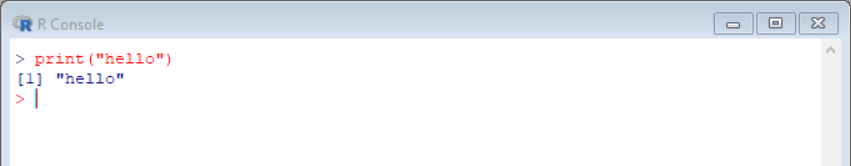
\includegraphics[width=0.85\textwidth]{figures/R-console-r}
  \caption[The R console]{The \Rpgrm console where the user can type textual commands one by one. Here the user has typed \code{print("Hello")} and \textit{entered} it by ending the line of text by pressing the ``enter'' key. The result of running the command is displayed below the command. The character at the head of the input line, a ``$>$'' in this case, is called the command prompt, signalling where a command can be typed in. Commands entered by the user are displayed in red, while results returned by R are displayed in blue.}\label{fig:intro:console}
\end{figure}

The \Rpgrm program does not have a graphical user interface (GUI), or menus from which to start different types of analyses. Instead, the user types the commands at the \Rpgrm console (Figure \ref{fig:intro:console}). The commands can be also saved into a text file, line by line, and such the file, called a `script' can substitute repeated typing of the same sequence of commands. When we work at the console typing in commands one by one, we say that we use R interactively. When we run script we may say that we run a ``batch job''.

The two approaches described above are part of the \Rpgrm program by itself. However, it is common to use a second program as a front-end or middle man ``in-between'' the user and the \Rpgrm program. Such a program allows more flexibility and has multiple features that makes entering commands or writing scripts easier---in other words makes it easier for the user to interact with \Rpgrm. Computations are still done by exactly the same \Rpgrm program. The simplest option is to use a text editor like \pgrmname{Emacs} to edit the scripts and then run the scripts in \Rpgrm from within the editor. With some editors like \pgrmname{Emacs}, rather good integration is possible. However, nowadays there are also Integrated Development Environments (IDEs) available for \Rpgrm. An IDE gives access to both use of the \Rpgrm console in a window, and provides a text editor for writing scripts in a separate window. Of the available IDEs for \Rpgrm, \RStudio is currently the most popular by a wide margin.

\subsubsection{Using R interactively}

A physical terminal (keyboard plus text-only screen) decades ago was how users communicated with computers, and was frequently called \emph{console}\index{console}. Nowadays, a text-only interface to a computer, in most cases a window or a pane within a graphical user interface it is still called a console. In our case, the \Rpgrm console (Figure \ref{fig:intro:console}). This is the native user interface of \Rpgrm.

Typing commands at the \Rpgrm console is useful when one is playing around, rather aimlessly exploring things, or trying to understand how an \Rpgrm function or operator we are not familiar with works. Once we want to keep track of what we are doing, there are better ways of using \Rpgrm, which allow us to keep a record of how an analysis has been carried out. The different ways of using \Rpgrm are not exclusive of each other, so most users will use the \Rpgrm console to test individual commands and plot data during the first stages of exploration. As soon as we decide how we want to plot or analyse the data, it is best to start using scripts. This is not enforced in any way by \Rpgrm, but scripts are what really brings to light the most important advantages of using a programming language for data analysis. In Figure \ref{fig:intro:console} we can see how the \Rpgrm console looks. The text in red has been typed in by the user---except for the prompt \code{$>$}---, and the text in blue is what \Rpgrm has displayed in response. It is essentially a dialogue between user and \Rpgrm. The console can \emph{look} different when displayed within an IDE like \RStudio, but the only difference is in the appearance of the text rather than in the text itself (cf.\ Figures \ref{fig:intro:console} and \ref{fig:intro:console:rstudio}).

\begin{figure}
  \centering
  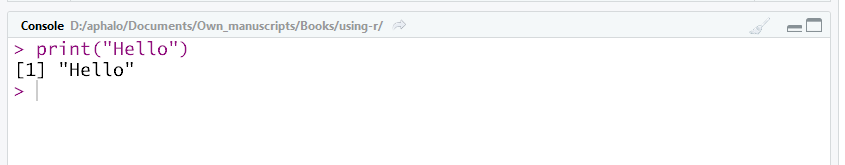
\includegraphics[width=\linewidth]{figures/r-console-rstudio}
  \caption[The R console]{The \Rpgrm console embedded in \RStudio. The same commands have been typed-in as in Figure \ref{fig:intro:console}. Commands entered by the user are displayed in purple, while results returned by \Rpgrm are displayed in black.}\label{fig:intro:console:rstudio}
\end{figure}

The two previous figures showed the result of entering a single command. Figure \ref{fig:intro:console:capture} shows how the console looks after the user has entered several commands, each as a separate line of text.

\begin{figure}
  \centering
  \includegraphics[width=\linewidth]{figures/r-console-capture}
  \caption[The R console]{The \Rpgrm console after several commands have been entered. Commands entered by the user are displayed in red, while results returned by \Rpgrm are displayed in blue.}\label{fig:intro:console:capture}
\end{figure}

The examples in this book require only the console window for user input. Menu-driven programs are not necessarily bad, they are just unsuitable when there is a need to set very many options and choose from many different actions. They are also difficult to maintain when extensibility is desired, and when independently developed modules of very different characteristics need to be integrated. Textual languages also have the advantage, to be dealt in later chapters, that command sequences can be stored in human- and computer readable text files. Such files constitute a record of all the steps used and in most cases makes it trivial to reproduce the same steps at a later time. Scripts are also a very simple and handy way of communicating to others how to do a given data analysis. When working at the command prompt, most results are printed by default, but in within scripts one needs to use the function \Rfunction{print()} explicitly.

\begin{explainbox}
In the console one types commands at the \code{>} prompt. When one ends a line by pressing the return or enter key, if the line can be interpreted as an R command, the result will be printed at the console, followed by a new \code{>} prompt.
If the command is incomplete a \code{+} continuation prompt will be shown, and you will be able to type-in the rest of the command. For example if the whole calculation that you would like to do is $1 + 2 + 3$, if you enter in the console \code{1 + 2 +} in one line, you will get a continuation prompt where you will be able to type \code{3}. However, if you type \code{1 + 2}, the result will be calculated, and printed.
\end{explainbox}

\subsubsection{Using R as a ``batch job''}

To run a script we need first to prepare a script in a text editor. Figure \ref{fig:intro:script} shows the console immediately after running the script file shown in the text editor. As before, red text, the command \code{source("my-script.R")}, was typed by the user, and the blue text in the console is what was displayed by \Rpgrm as a result of this action. The title bar of the console, shows ``R-console'', while the title bar of the editor shows the \emph{path} to the script file that is open and ready to be edited followed by ``R-editor''.

\begin{figure}
  \centering
  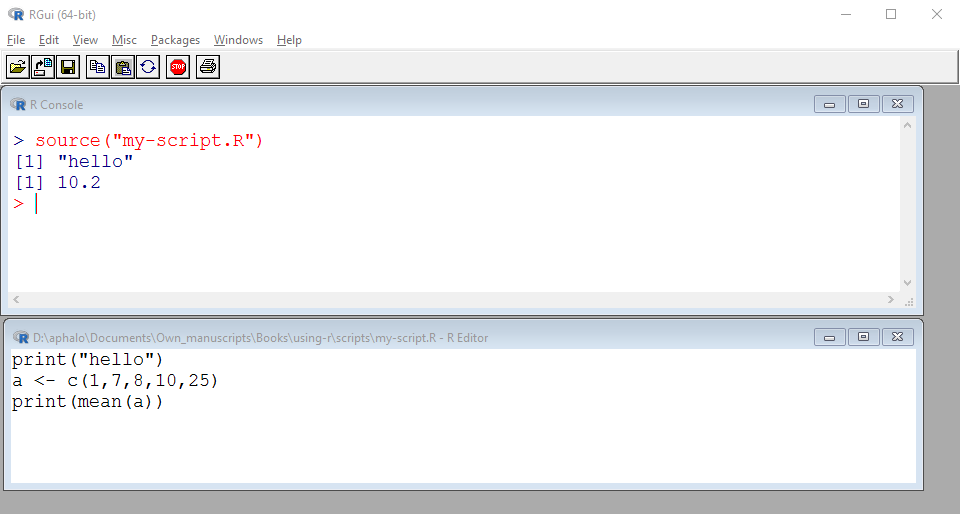
\includegraphics[width=\linewidth]{figures/R-console-script}
  \caption[Script sourced at the R console]{Screen capture of the \Rpgrm console and editor just after running a script. The upper pane shows the \Rpgrm console, and the lower pane the script file in an editor. }\label{fig:intro:script}
\end{figure}

A true ``batch job'' is not run at the \Rpgrm console but at the operating system command prompt, or shell. The shell is the console of the operating system---\osname{Linux}, \osname{Unix}, \osname{OS X}, or \osname{MS-Windows}. Figure \ref{fig:intro:shell} shows how running an script at the Windows command prompt looks. A script can be run at the operating system prompt to do time-consuming calculations with the output saved to a file. One may use this approach on a server, say, to leave a large data analysis job running over-night or for even several days.

\begin{figure}
  \centering
  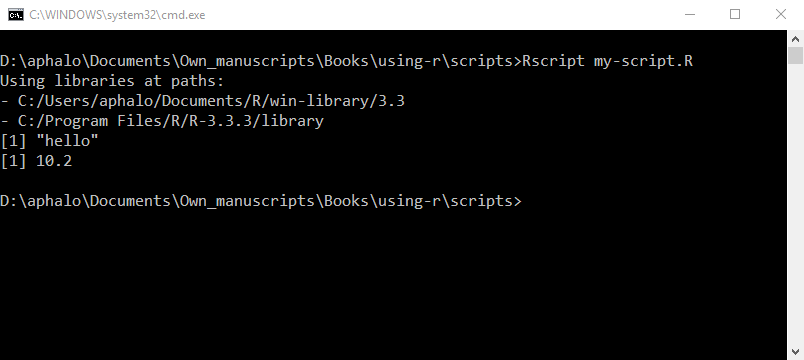
\includegraphics[width=\linewidth]{figures/windows-cmd-script}
  \caption[Script at the Windows cmd promt]{Screen capture of the \osname{MS-Windows} command console just after running the same script. Here we use \code{Rscript} to run the script, the exact syntax will depend on the operating system in use. In this case \Rpgrm prints the results at the operating system console or shell, rather than in its own \Rpgrm console.}\label{fig:intro:shell}
\end{figure}

Batch jobs are not the only, or main use of scripts, as they are useful even in data analysis jobs that take just seconds to run as they provide a way of keeping a faithful record of the steps that have been followed from data input to final analysis and graphical presentation.

\subsubsection{Editors and IDEs}

Integrated Development Environments (IDEs) are used when developing computer programs. IDEs provide a centralized user interface from within which the different tools used to create and test a computer program can be accessed and used in coordination. Most IDEs include a dedicated editor capable of syntax highlighting, and even report some mistakes, related to the programming language in use. One could describe such editor as the equivalent as a word processor with spelling and grammar checking, that can alert about spelling and syntax errors for a computer language like \Rlang instead of for a natural language like English. In the case of \RStudio, the main, but not only language supported is \Rlang. \RStudio in contrast to other IDEs targets also data analysis. The main window of IDEs usually displays more than one pane simultaneously. From within the \RStudio IDE one has access to the \Rpgrm console, a text editor, a file-system browser, a pane for graphical output, and access to several additional tools such the installation of extension packages. Although \RStudio supports very well the development of large scripts and packages, it is also the best possible way of using \Rpgrm at the console as it has the \Rpgrm help system very well integrated both in the editor and R console. Figure \ref{fig:intro:rstudio} shows the main window displayed by \RStudio after running the same script as shown above at the \Rpgrm console (Figure \ref{fig:intro:script}) and at the operating system command prompt (Figure \ref{fig:intro:shell}). We can see by comparing these three figures how \RStudio is really a layer between the user and an unmodified \Rpgrm executable. The script was sourced by pressing the ``Source'' button at the top of the editor pane. \RStudio in response to this generated the code needed to source the file and ``entered'' it at the console, the same console, where we would type ourselves any \Rpgrm commands.

\begin{figure}
  \centering
  \includegraphics[width=\linewidth]{figures/Rstudio-script}
  \caption[Script in Rstudio]{The \RStudio interface just after running the same script. Here we used the ``Source'' button to run the script. In this case \Rpgrm prints the results to the \Rpgrm console in the lower left pane.}\label{fig:intro:rstudio}
\end{figure}

When a script is run, if an error is triggered, \RStudio automatically finds the location of the error. \RStudio also supports the concept of projects allowing saving of settings per project. Some features are beyond what you need for everyday data analysis and aimed at package development, such as integration of debugging, traceback on errors, profiling and bench marking of code so as to analyse and improve performance. It also integrates support for file version control, which is not only useful for package development, but also for keeping track of the progress or collaboration in the analysis of data.

The version of \RStudio that one uses locally, i.e.\ installed in a computer used locally by a single user, runs with almost identical user interface on most modern operating systems, such as \osname{Linux}, \osname{Unix}, \osname{OS X}, and \osname{MS-Windows}. There is also a server version that runs on \osname{Linux}, and that can be used remotely through a web browser. The user interface is still the same.

\RStudio is under active development, and constantly improved. Visit \url{http://www.rstudio.org/} for an up-to-date description and download and installation instructions. Two books \autocite{vanderLoo2012,Hillebrand2015} describe and teach how to use \RStudio without going in depth into data analysis or statistics, however, as \RStudio is under very active development several recently added important features are not described in these books. You will find tutorials and up-to-date cheat sheets at \url{http://www.rstudio.org/}.

\section{Packages and repositories}
\index{packages!extending R}
The most elegant way of adding new features or capabilities to \Rlang is through packages. This is without doubt the best mechanism when these extensions to \Rlang need to be shared. However, in most situations it is also the best mechanism for managing code that will be reused even by a single person over time. \Rlang packages have strict rules about their contents, file structure, and documentation, which makes it possible among other things for the package documentation to be merged into \Rpgrm's help system when a package is loaded. With a few exceptions, packages can be written so that they will work on any computer where \Rpgrm runs.

Packages can be shared as source or binary package files, sent for example through e-mail. However, for sharing packages widely, best is to submit them to a repository. The largest public repository of \Rpgrm packages is called CRAN\index{CRAN}, an acronym for Comprehensive R Archive Network. Packages available through CRAN are guaranteed to work, in the sense of not failing any tests built into the package and not crashing or aborting prematurely. They are tested daily, as they may depend on other packages whose code will change when updated. In January 2017, the number of packages available through CRAN passed the 10\,000 mark.

Using packages requires in general two steps: 1) installing the package into the \Rpgrm library\index{packages!library}\index{packages!installation} and 2) loading it from the library into the current \Rpgrm session\index{packages!loading}. Installation is needed once and consists in making a local copy of the package, i.e.\ in the hard disk. Loading needs to be done at least once in each \Rpgrm session, and before any command defined in the package can be used. Loading a package also loads the corresponding help pages.

Packages are installed into the library using function \Rfunction{install.packages()} and are loaded from the library with function \Rfunction{library()}.

\begin{playground}
  Use \code{help} to look up the help pages for \code{install.packages} and \code{library}, and explain what the code in the next chunk does.
\begin{knitrout}\footnotesize
\definecolor{shadecolor}{rgb}{0.969, 0.969, 0.969}\color{fgcolor}\begin{kframe}
\begin{alltt}
\hlkwd{install.packages}\hlstd{(learnrbook)}
\hlkwd{library}\hlstd{(learnrbook)}
\hlkwd{help}\hlstd{(learnrbook)}
\end{alltt}
\end{kframe}
\end{knitrout}
\end{playground}

When using an IDE like \RStudio, although these commands can be typed into the \Rpgrm console, it is usually easier to manage installation and update of packages through the IDE's interface, which in turn generates the needed \Rlang code and runs it in the console.

Loading of packages seems to me easier directly at the console or as part of a script. Of course, this is my own preference that may differ from yours!

\section{Reproducible data analysis}
\index{reproducible data analysis|(}
Reproducible data analysis is much more than a fashionable buzzword. Under any situation where accountability is important, from scientific research to decision making in commercial enterprises, industrial quality control and safety and environmental impact assessments, being able to reproduce a data analysis reaching the same conclusions from the same data is crucial. Most approaches to reproducible data analysis are based on automating report generation and including as part of the report all the computer commands used to generate the results presented.

A fundamental requirement for reproducibility, is a reliable record of what commands have been run on which data. Such a record is specially difficult to keep when issuing commands through menus and dialogue boxes in a graphical user interface or interactively at a console. Even working interactively at the \Rpgrm console using copy and paste to include commands and results in a report is error prone, and laborious.

A further requirement is to be able to match the output of the \Rlang commands to the input. If the script saves the output to separate files, then the user will need to take care that the script saved or shared as record of the data analysis was the one actually used for obtaining the reported results and conclusions. This is another error prone stage in the reporting of a data analysis. To solve this problem an approach was developed, inspired in what is called \emph{literate programming} \autocite{Knuth1984a}. The idea is that running the script will produce a document that includes the script, the results of running the scripts and any explanatory text needed to understand and interpret the analysis.

Although a system capable of producing such reports with \Rlang, called \pkgname{Sweave} \autocite{Leisch2002}, has been available for a couple decades, it was rather limited and not supported by an IDE, making its use rather tedious. A more recently developed system called \pkgname{knitr} \autocite{Xie2013} together with its integration into \RStudio has made the use of this type of reports very easy. The most recent development is what has been called \Rlang \emph{notebooks} produced within \RStudio. This new feature, can produce the readable report of running the script as an HTML file, displaying the code used interspersed with the results within the viewable file as in earlier approaches. However, this newer approach goes even further: the actual source script used to generate the report is embedded in the HTML file of the report and can be extracted and run very easily and consequently re-used. This means that anyone who gets access to the output of the analysis in human readable form also gets access to the code used to generate the report, in computer executable format.

Because of these recent developments, \Rlang is an ideal language to use when the goal of reproducibility is important. During recent years the problem of the lack of reproducibility in scientific research has been broadly discussed and analysed \autocite{Gandrud2015}. One of the problems faced when attempting to reproduce experimental work, is reproducing the data analysis. \Rlang together with these modern tools can help in avoiding this source of lack of reproducibility.

How powerful are these tools? and how flexible? They are powerful and flexible enough to write whole books, such as this very book you are now reading, produced with \Rpgrm, \pkgname{knitr} and \LaTeX\index{Latex@\LaTeX}. All pages in the book are generated directly, all figures are generated by \Rpgrm and included automatically, except for the figures in this chapter that have been manually captured from the computer screen. Why am I using this approach? First because I want to make sure that every bit of code as you will see printed, runs without error. In addition I want to make sure that the output that you will see below every line or chunk of \Rlang language code is exactly what \Rpgrm returns. Furthermore, it saves a lot of work for me as author, as I can just update \Rpgrm and all the packages used to their latest version, and build the book again, to keep it up to date and free of errors.

Although the use of these tools is important, they are outside the scope of this book and well described in other books \autocite{Gandrud2015,Xie2013}. Still when writing code, using a consistent style for formatting and indentation, carefully choosing variable names, and adding textual explanations in comments when needed, helps very much with readability for humans. I have tried to be as consistent as possible throughout the whole book in this respect, with only small personal deviations from the usual style.
\index{reproducible data analysis|)}

\section{Finding additional information}

When searching for answers, asking for advice or reading books you will be confronted with different ways of approaching the same tasks. Do not allow this to overwhelm you, in most cases it will not matter as many computations can be done in \Rpgrm, as in any language, in several different ways, still obtaining the same result. The different approaches may differ mainly in two aspects: 1) how readable to humans are the instructions given to the computer as part of a script or program, and 2) how fast the code runs. Unless computation time is an important bottleneck in your work, just concentrate on writing code that is easy to understand to you and to others, and consequently easy to check and reuse. Of course do always check any code you write for mistakes, preferably using actual numerical test cases for any complex calculation or even relatively simple scripts. Testing and validation are extremely important steps in data analysis, so get into this habit while reading this book. Testing how every function works as I will challenge you to do in this book, is at the core of any robust data analysis or computing programming.

\begin{warningbox}
Error messages tend to be terse in \Rpgrm, and may require some lateral thinking and/or `experimentation' to understand the real cause behind problems. When you are not sure to understand how some command works, it is useful in many cases to try simple examples for which you know the correct answer and see if you can reproduce them with \Rpgrm. Because of this, this book also includes some code examples that trigger errors. Learning to interpret error messages is part of what is needed to become a proficient user of \Rlang. To test your understanding of how a code statement or function works, it is good to try your hand at testing its limits, testing which variations of a piece code are valid or not.
\end{warningbox}

\subsection{R's built-in help}

To\index{R!help} access help pages through the command prompt we use function \Rfunction{help()} or a question mark. Every object exported by an \Rlang package (functions, methods, classes, data) is documented. Sometimes a single help page documents several \Rlang objects. Usually at the end of the help pages, some examples are given, which tend to help very much in learning how to use the functions described. For example one can search for a help page at the \Rpgrm console.

\begin{knitrout}\footnotesize
\definecolor{shadecolor}{rgb}{0.969, 0.969, 0.969}\color{fgcolor}\begin{kframe}
\begin{alltt}
\hlkwd{help}\hlstd{(}\hlstr{"sum"}\hlstd{)}
\hlopt{?}\hlstd{sum}
\end{alltt}
\end{kframe}
\end{knitrout}

\begin{playground}
Look at help for some other functions like \code{mean()}, \code{var()}, \code{plot()} and, why not, \Rfunction{help()} itself!
\begin{knitrout}\footnotesize
\definecolor{shadecolor}{rgb}{0.969, 0.969, 0.969}\color{fgcolor}\begin{kframe}
\begin{alltt}
\hlkwd{help}\hlstd{(help)}
\end{alltt}
\end{kframe}
\end{knitrout}
\end{playground}

When using \RStudio there are easier ways of navigating to a help page than using function \Rfunction{help()}, for example with the cursor on the name of a function in the editor or console, pressing the F1 key, opens the corresponding help page in the help pane. Letting the cursor hover for a few seconds over the name of a function at the \Rpgrm console will open ``bubble help'' for it. If the function is defined in a script or another file open in the editor pane one can directly navigate from the line where the function is called to where it is defined. In \RStudio one can also search for help through the graphical interface.

In addition to help pages, the \Rpgrm's distribution includes useful manuals as PDF or HTML files. These can be accessed most easily through the Help menu in \RStudio or \pgrmname{RGUI}. Extension packages, provide help pages for the functions and data they export. When a package is loaded into an \Rpgrm session, its help pages are added to the native help of \Rpgrm. In addition to these individual help pages, each package, provides an index of its corresponding help pages, for users to browse. Many packages, also provide \emph{vignettes} such as User Guides or articles describing the algorithms used.

There are some web sites that give access to \Rlang documentation through a web server. These sites can be very convenient when exploring whether a certain package could be useful for a certain problem, as they allow browsing and searching the documentation without need of installing the packages. Some package maintainers have web sites with additional documentation for their own packages. The DESCRIPTION or README of packages provide contact information for the maintainer, links to web sites, and instructions on how to report bugs. As packages are contributed by independent authors, they should be cited in addition to citing \Rpgrm itself. \Rlang function \code{citation()} with the name of a package as argument provides the reference that should be cited, and without an explicit argument, the reference to use for the version of \Rlang in use.

\begin{knitrout}\footnotesize
\definecolor{shadecolor}{rgb}{0.969, 0.969, 0.969}\color{fgcolor}\begin{kframe}
\begin{alltt}
\hlkwd{citation}\hlstd{()}
\end{alltt}
\begin{verbatim}
## 
## To cite R in publications use:
## 
##   R Core Team (2018). R: A language and environment for
##   statistical computing. R Foundation for Statistical Computing,
##   Vienna, Austria. URL https://www.R-project.org/.
## 
## A BibTeX entry for LaTeX users is
## 
##   @Manual{,
##     title = {R: A Language and Environment for Statistical Computing},
##     author = {{R Core Team}},
##     organization = {R Foundation for Statistical Computing},
##     address = {Vienna, Austria},
##     year = {2018},
##     url = {https://www.R-project.org/},
##   }
## 
## We have invested a lot of time and effort in creating R, please
## cite it when using it for data analysis. See also
## 'citation("pkgname")' for citing R packages.
\end{verbatim}
\end{kframe}
\end{knitrout}

\begin{playground}
  Look at the help page for function \code{citation()} for a discussion of why it is important for users to cite \Rpgrm and packages when using them.
\end{playground}

\subsection{Obtaining help from on-line forums}

When consulting help pages, vignettes and possibly books at hand fails to provide the information the next step to follow is to search internet forums for existing answers to one's questions. When these steps fail to solve a problem, then it is time to ask for help, either from local experts or by posting your own question in a suitable on-line forum. When posting requests for help one needs to abide to what is usually described as ``netiquette''.

\subsubsection{Netiquette}
In\index{netiquette}\index{network etiquette} most internet forums, a certain behaviour is expected from those asking and answering questions. Some types of miss-behavior, like use of offensive or inappropriate language, will usually result in the user losing writing rights in a forum. Occasional minor miss-behaviour, will usually result in the original question not being answered and instead the problem highlighted in the reply. In general following the steps listed below will greatly increase your chances of getting a detailed and useful answer.

\begin{itemize}
  \item Do your homework: first search for existing answers to your question, both on-line and in the documentation. (Do mention that you attempted this without success when you post your question.)
  \item Provide a clear explanation of the problem, and all the relevant information. Say if it concerns \Rpgrm, the version, operating system, and any packages loaded and their versions.
  \item If at all possible provide a simplified and short, but self-contained, code example that reproduces the problem (sometimes called \emph{reprex}).
  \item Be polite.
  \item Contribute to the forum by answering other users' questions when you know the answer.
\end{itemize}

\subsubsection{StackOverflow}

Nowadays, StackOverflow (\url{http://stackoverflow.com/})\index{StackOverflow} is the best questions and answers (Q\,\&\,A) support site for \Rpgrm. In most cases, searching for existing questions and their answers, will be all what you need to do. If asking a question, make sure that it is really a new question. If there is some question that looks similar, make clear how your question is different.

StackOverflow has a user-rights system based on reputation, and questions and answers can be up- and down-voted. Those with the most up-votes are listed at the top of searches. If the questions or answers you write are up-voted after you accumulate enough reputation you acquire badges, and rights, such as editing other users' questions and answers or later on, even deleting wrong answers or off-topic questions from the system. This sounds complicated, but works extremely well at ensuring that the base of questions and answers is relevant and correct, without relying on a single or ad-hoc \emph{moderators}.

\subsubsection{Reporting bugs}

Being careful in the preparation of a reproducible example\index{reproducible example}\index{reprex|see{reproducible example}} is specially important when you intend to report a bug to the maintainer of any piece of software. For the problem to be fixed, the person revising the code, needs to be able to reproduce the problem, and after modifying the code, needs to be able to test if the problem has been solved or not. However, even if you are facing a problem caused by your misunderstanding of how \Rlang works, the simpler the example, the more likely that someone will quickly realize what was your intention when writing the code that produces a result different from what you expected.

\begin{explainbox}
How to prepare a reproducible example\index{reproducible example} (``reprex''). A \emph{reprex} is a self-contained and as simple as possible piece of computer code that triggers (and so demonstrates) a problem. If possible when you need to use data, either use a data set included in base \Rpgrm or generate artificial data within the reprex code. If you can reproduce the problem only with your own data, then you need to provide a minimal subset of it that triggers the problem.

While preparing the \emph{reprex} you will need to simplify the code, and sometimes this already makes a diagnose by yourself much likely. In general, before, posting a reprex on-line, it is wise to check it with the latest versions of \Rpgrm and any package being used.

I would say that about two out of three times I start preparing a \emph{reprex}, preparing the \emph{reprex} allows me to much better understand the problem and find the root of the problem or a work-around on my own.
\end{explainbox}

\section{What is needed to run the examples in this book?}

The book is written with the expectation that you will run most of the code examples and try as many other variations as needed until you are sure to understand the basic `rules' of the \Rpgrm language and how each function or command described works. As mentioned above, you are expected to use this book as a travel guide for your exploration of the world of \Rlang.

\Rpgrm is all what is needed to work through all the examples in this book, but it is not a convenient way of doing this. I recommend you to use an editor or an IDE, in particular \RStudio\index{IDE for R}\index{editor for R scripts}. \RStudio is user friendly, actively maintained, free, open-source and available both in desktop and server versions. The desktop version runs on \osname{MS-Windows}, \osname{Linux}, and \osname{OS X} and other \osname{Unix} distributions.

Of course when choosing which editor to use, personal preferences and previous familiarity play an important role.
Currently, for the development of packages, I use \RStudio exclusively. For writing this book I have used both \RStudio and the text editor \pgrmname{WinEdt} which also has support for \Rpgrm together with excellent support for \LaTeX\index{Latex@\LaTeX}. When working on a large project or collaborating with other data analysts or researchers, one big advantage of a system based on plain text files such as R scripts, is that the same files can be edited with different programs and under different operating systems as needed or wished by the different persons involved in a project.

When I started using \Rpgrm, nearly two decades ago, I was using other editors, using the operating system shell a lot more, and struggling with debugging as no IDE was available. The only reasonably good integration with an editor was for \pgrmname{Emacs}, which was widely available only under \osname{Unix}-like systems. Given my past experience, I encourage you to use an IDE for \Rpgrm. \RStudio is nowadays very popular, but if you do not like it, need a different set of features, such as integration with \pgrmname{ImageJ}, or are already familiar with the \pgrmname{Eclipse} IDE, you may want to try the \pgrmname{Bio7} IDE, available from \url{http://bio7.org}.

The examples in this book make use of several freely available packages, which can be installed from CRAN. One of them \pkgname{learnrbook} also available through CRAN, contains data sets and files specific to this book. The \pkgname{learnrbook} package also contains installation instructions and saved lists of the names of all other packages used in the book. Instructions on installing \Rpgrm, \pgrmname{Git}, \RStudio, compilers and other tools are available on-line. In many cases the IT staff at your employer or school will know how to install them, or they may be even included in the default computer setup. In addition a web site supporting the book will be available at: \url{http://www.learnr-book.info}.




























